\section{Wordnet}


\subsection{Ontologien im NLP}

Bei der zwischenmenschlichen Kommunikation werden Informationen in codierter Form über das Medium der Sprache übertragen. Für den Erfolg des Informationstausches ist die richtige Decodierung der abstrakten Spracheinformationen, das heißt die richtige Verknüpfung eines Wortes mit dessen Bedeutung, entscheidend. 
\begin{quote} \textit{"`In order to effectively exchange information, agents need to share a lexicon of words as well as to access the world model(s) underlying the lexicon."'} (\cite[vgl.][1]{OLTRAMANI})\end{quote} 
Die Kommunikationspartner müssen sowohl über denselben Wortschatz als auch über ein gemeinsames Weltverständnis (engl. \textit{world model}) verfügen. Dies gilt auch für die Mensch-Maschine Kommunikation. Ein World Model kann beispielsweise mittels einer Ontologie in maschinenlesbarer Form abgebildet werden. Eine Ontologie ist in der Informatik definiert als System von Informationen mit logischen Relationen (\cite[vgl.][1]{DUDEN}). Eingeführt wurde der Begriff in de 1970er Jahren auf dem Forschungsgebiet der künstlichen Intelligenz zur Modellierung von Wissen. Ziel von digitalen Ontolgien ist es, Wissensdomänen in maschinenlesbarer Form verfügbar zu machen (\cite[vgl.][7]{TACKE}). Somit sind Ontologien eine zentrale Komponente in Wissenssystemen. 
\par
Das \textit{Princeton WordNet} ist eine solche Ontologie, also eine als semantisches Netz organisierte, lexikalische Ressource. Die Entwicklung von WordNet begann bereits 1985 and der Universität Princeton. 1993 wurde die erste Version veröffentlicht. Die aktuelle Version, das \textit{WordNet 3.0}, enthält etwa 155.000 manuell verfasste Einträge in englischer Sprache. (\cite[vgl.][1]{PRINCETON})
\par
Die aktuelle Version folgt außerdem den Linked Open Data Principles, und somit auch den Grundsätzen des Semantic Web. 
\par
\textit{„Linked Open Data (LOD) is Linked Data which is released under an open licence, which does not impede its reuse for free.“}(\cite[vgl.][1]{BERNERS_LEE}). 
\par
Die freie Verfügbarkeit und die Linked-Data-Struktur haben maßgeblich zur weiten Verbreitung von WordNet beigetragen. Als Metadatenformat in Wordnet wurde die weit verbreitete, standardisierte \textit{Web Ontology Language} eingesetzt. Im \ac{NLP} wird auf WordNet für die Erstellung der semantischen Annotationen benötigt. Es dient als essentielle Ressource für überwacht lernende Algorithmen.
\par

\subsection{Aufbau und Struktur}

DIe Basiseinheit in WordNet ist das WOrt in seiner Grundform (Lemma). In WordNet werden Wörter mit gleicher oder nahezu identischer Bedeutung in Synsets gruppiert. Der Begriff ist ein Neologismus aus \textit{synonym} (dt. Synonym) und \textit{set} (dt. Menge, Zusammenstellung). Die Synsets werden über Kanten verknüpft, die bestimmte semantische Relationen repräsentieren. So entsteht ein gerichteter azyklischer Graph (\cite[vgl.][12]{OLTRAMANI}), der dem Aufbau des neuronalen Netzes im menschlichen Gehirn ähnelt.Grundsätzlich setzt sich WordNet aus vier Datenbanken für die jeweiligen Wortarten Nomen, Verben, Adjektive und Adverben zusammen. Jede dieser Datenbanken beinhaltet miteinander verknüpfte Synsets. Hierbei wird jeweils auch die Arte der Verknüpfung bzw. der semantischen Relation angegeben. Abhängig von der Wortart sind verschiedene Arten von Relationen möglich. Tabelle \ref{table:table2} zeigt die Relationen von Nomen und Verben in WordNet geordnet nach Häufigkeit.
\par
\begin{table}[h!]
  \centering
  \begin{tabular}{ccccc} %Hier muss für jede Spalte ein c hin -> Dump wegen mismatch von definierter und auftretender Spaltenanzahl
    \toprule
     Rang & Relationen der Nomen & Anteil  & Relationen der Verben & Anteil \\
    \midrule
    1 & Hyponyme/Hypernyme: & 45.5\% & Abgeleitete Form:    & 55.4\% \\
    2 & Abgeleitete Form:   & 22.4\% & Troponyme/Hypernyme: & 31.7\% \\
    3 & Meronyme/Holonymy:  & 13.3\% & Verbgruppe:          & 4.2\%  \\
    4 & Wissensgebiet:      & 9.1\%  & Wissensgebiet:       & 3.0\%  \\
    5 & Typ/Instanz: 		& 5.1\%  & Antonymy:			& 2.6\%  \\
    6 & Pertainyme: 		& 2.9\%  & Siehe auch: 		    & 1.4\%  \\
    7 & Antonyme: 			& 1.3\% & Folgebeziehung: 	    & 1.0\%  \\
	8 & Attribut: 			& 0.4\%  & Ursache: 			& 0.5\%  \\
	9 & Partizip: 	        & 0.2\%  & -     	            & -  	 \\
	\bottomrule
  \end{tabular}
  \caption{Relationen in WordNet (\cite[vgl.][9]{MAZIARZ})}
  \label{table:table2}
\end{table}
\par

Der bei Nomen am häufigsten auftretende Beziehungstyp ist das Hyponym/Hypernym. Diese Beziehung strukturiert die Synsets hierarchisch in übergordnete Elter-Synsets (Hypernym) und untergeordnete Kind-Synsets (Hyponym). Es handelt sich also um eine IS-A-Beziehung. Das äquivalent zu Hyponymen in der Kategorie Verben wird als Troponym bezeichnet. Abgleitete Formen verbinden Synsets über Wortarten-Grenzen hinweg. Beispielsweise ist das Verb \textit{run} mit dem Nomen \textit{run} über die Beziehung der abgeleiteten Form verbunden. Ein weiterer häufiger Beziehungstyp sind Meronyme- und Holonyme-Beziehungen. Sie stellen die Part-Of-Beziehung (Meronym) und deren Gegenstück dar.

\par
\subsection{Word Sense Disambiguation}

Die meisten Worte einer Sprache haben mehrere Bedeutungen. Die richtige Wortbedeutung ergibt sich folglich erst aus dem Kontext der Wortverwendung. Um die Wortbedeutung maschinell zu erfassen, sind ein \textit{Sense Inventory} und ein klassifizierender Algorithmus notwendig. 
\begin{figure}[h]
\begin{center}
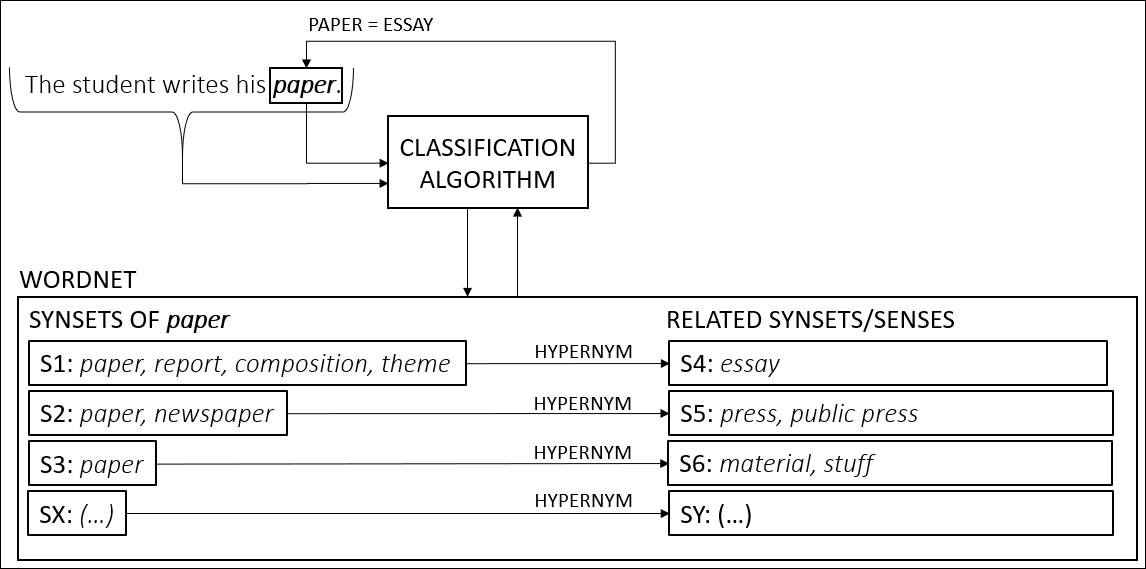
\includegraphics[keepaspectratio=true, width=\textwidth]{pictures/WSD.png}
\caption{WSD Klassifikation mit WordNet (eigene Darstellung)}
\label{fig:WSD}
\end{center}
\end{figure}
Bei einem solchen Sense Inventory handelt es sich um eine Informationsquelle, in der die verschiedenen Wortbedeutungen einsehbar sind. WordNet kann diese Rolle übernehmen. Ein mehrdeutiges Wort ist in WordNet Mitglied in verschiedenen Synsets, aus deren hypernymen Synsets sich dann die verschiedenen Wortbedeutungen ableiten lassen. Abbildung \ref{fig:WSD} zeigt einen Beispielsatz, indem die Bedeutung des englischen Wortes \textit{paper} ermittelt werden soll.
\par 
Der Klassifikationsalogrithmus, hier als Blackbox dargestellt, nutzt die hierarchische Struktur von WordNet um die verschiedenen Bedeutungen nachzuschlagen. Daraufhin wählt er die wahrscheinlichste Bedeutung im Satzzusammenhang aus. In diesem Fall wählt er korrekt die Bedeutung \textit{essay} aus.
\par
Somit ist Word Sense Disambiguation nichts anderes als ein Klassifikationsproblem, das basierend auf gewissen Eingabeparametern eine Einordnung vornimmt. Prinzipiell kann jeder generische, maschinell lernende Klassifikationsalgorithmus zur Lösung herangezogen werden (\cite[vgl.][326]{YAROWSKY}). Als am verlässlichsten stellen jedoch Kombinationen verschiedener Ranking-Algorithem heraus. Die geringe Menge an verfügbaren Trainingsdaten stellt hierbei jedoch immernoch ein Problem dar.


\subsection{Java APIs}

Um WordNet direkt in eigene Softwareprojekte einbinden zu können, stehen allein für die Programmiersprache Java zwölf verschiedenen Bibliotheken zu Verfügung. Bei der Wahl einer geeigneten Bibliothek hängt von verschiedenen Faktoren ab. Im Vergleich schneidet das \textit{Java WordNet Interface} \ac{JWI} für den allgemeinen Anwendungsfall am besten ab (\cite[vgl.][2]{FINLAYSON}). Auch gegenüber der weit verbreiteten \textit{Java WordNet Library} \ac{JWNL} bietet es nach Finlayson die folgenden Vorteile:

\begin{itemize} 
\item Vollumfänglicher Zugriff auf alle WordNet Ressourcen
\item Arbeitet direkt mit den WordNet-Files (keine Modifizierung notwendig)
\item Dateibasierte und In-Memory-basierte Implementierungsmöglichkeiten
\item Anzahl der instanziierten Dictionaries kann beliebig groß gewählt werden
\item Sehr hohe Performanz, speicherschonend und unabhängig von anderen Systemen
\item Keine \textit{config-Datei} benötigt 
\item Ausführliche Dokumentation, aktiver Support und kontinuierliche Weiterentwicklung
\end{itemize}

Neben der direkten Einbindung von Wordnet über eine Java API, wird Wordnet auch von Standard-Software-Toolkits wie dem Standford CoreNLP oder dem NLTK als Informationsquelle genutzt.